\subsection{Sviluppatori}
\subsubsection{Panoramica sviluppatore}
\begin{figure}[H]
\centering
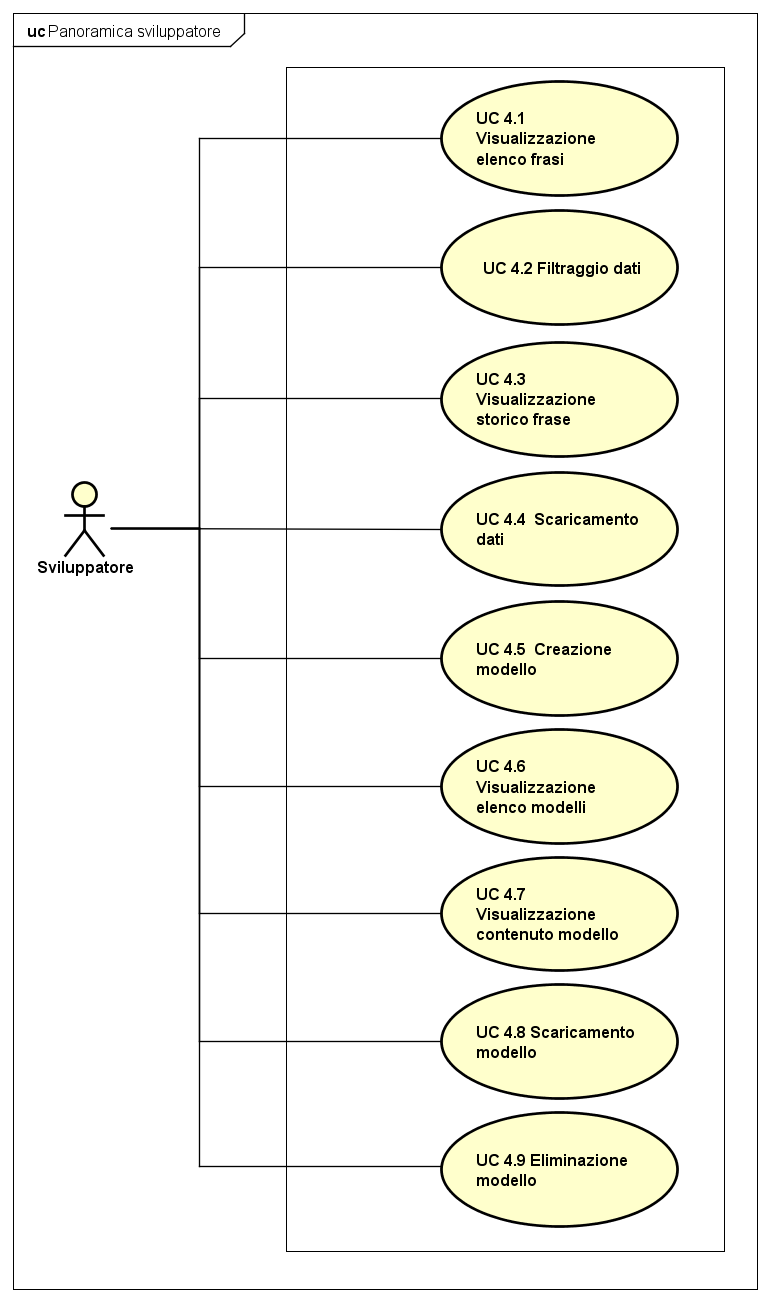
\includegraphics[width=17cm, height = 19cm]{img/UC4x.png} 
\caption{Panoramica sviluppatore}\label{fig:4x}
\end{figure}
\subsubsection{UC 4.1 - Visualizzazione elenco frasi}
\begin{itemize}
\item[•]\textbf{Attori}: Sviluppatore;
\item[•]\textbf{Descrizione}: lo sviluppatore visualizza un elenco di frasi accompagnate dalla data di creazione e dall’autore ordinate cronologicamente;
\item[•]\textbf{Precondizione}:  lo sviluppatore si è autenticato nel sistema;% e visualizza la propria dashboard\ped{G}.
\item[•]\textbf{Postcondizione}: lo sviluppatore visualizza l'elenco delle preposizioni ordinate cronologicamente;
\item[•]\textbf{Flusso degli eventi}: lo sviluppatore ha selezionato la voce relativa alla pagina contenente l’elenco delle frasi e ne visualizza il contenuto. 
\end{itemize}
\subsubsection{UC 4.2 - Filtraggio dei dati}
\begin{figure}[H]
\centering
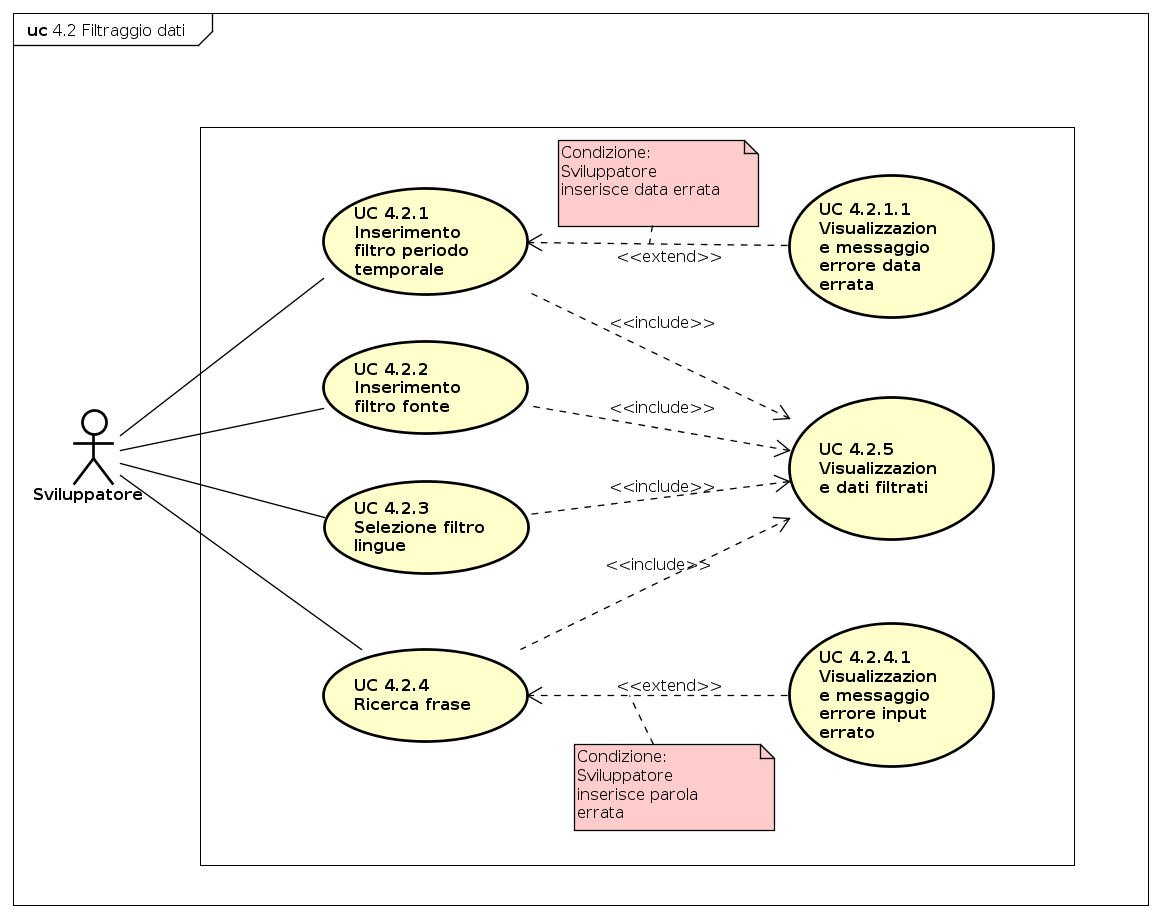
\includegraphics[width=17cm, height=10cm]{img/UC420.png} 
\caption{Caso d'uso UC 4.2}\label{fig:420}
\end{figure}
\begin{itemize}
\item[•]\textbf{Attori}: Sviluppatore;
\item[•]\textbf{Descrizione}: lo sviluppatore applica dei filtri ai dati, ottenendo solo quelli d'interesse;
\item[•]\textbf{Precondizione}: lo sviluppatore visualizza le proposizioni in ordine cronologico;
\item[•]\textbf{Postcondizione}: lo sviluppatore visualizza i dati che rispettano i filtri scelti;
\item[•]\textbf{Flusso degli eventi}:
\begin{enumerate}
\item UC 4.2.1 - Inserimento filtro periodo temporale;
\item UC 4.2.2 - Inserimento filtro {fonte}\ped{G};
\item UC 4.2.3 - Selezione filtro lingue;
\item UC 4.2.4 - Ricerca frase.
\end{enumerate}
\item[•]\textbf{Estensioni}:
\begin{enumerate}
	\item UC 4.2.6 - Rimozione filtro;
	\item UC 4.2.1.1 - Visualizzazione messaggio errore data errata;
	\item UC 4.2.4.1 - Visualizzazione messaggio errore input errato.
\end{enumerate}
\item[•]\textbf{Inclusioni}:
\begin{enumerate}
\item UC 4.2.5 - Visualizzazione dati filtrati.
\end{enumerate}
\end{itemize}
\subsubsection{UC 4.2.1 - Inserimento filtro periodo temporale}
\begin{itemize}
\item[•]\textbf{Attori}: Sviluppatore;
\item[•]\textbf{Descrizione}: lo sviluppatore seleziona un periodo temporale, ottenendo i dati salvati in un determinato arco di tempo;
\item[•]\textbf{Precondizione}: lo sviluppatore visualizza le proposizioni in base ai filtri stabiliti;
\item[•]\textbf{Postcondizione}: lo sviluppatore visualizza le frasi in base al filtraggio inserito;
\item[•]\textbf{Flusso degli eventi}: 
\begin{enumerate}
\item Scelta data inizio periodo;
\item Scelta data fine periodo.
\end{enumerate}
\item[•]\textbf{Estensioni}: 
\begin{enumerate}
	\item UC 4.2.1.1 - Visualizzazione messaggio errore data errata;
	\item UC 4.2.6 - Rimozione filtro.
\end{enumerate}
\item[•]\textbf{Inclusioni}:
\begin{enumerate}
\item UC 4.2.5 - Visualizzazione dati filtrati.
\end{enumerate}
\end{itemize}

\subsubsection{UC 4.2.2 - Inserimento filtro fonte}
\begin{itemize}
\item[•]\textbf{Attori}: Sviluppatore;
\item[•]\textbf{Descrizione}: lo sviluppatore seleziona una o più fonti degli esercizi, come ad esempio le correzione provenienti da determinati docenti o dal sistema di correzione automatico;
\item[•]\textbf{Precondizione}: lo sviluppatore visualizza le proposizioni in base ai filtri stabiliti;
\item[•]\textbf{Postcondizione}: lo sviluppatore ha impostato i valori del filtro fonte;
\item[•]\textbf{Flusso degli eventi}: lo sviluppatore seleziona da un elenco le fonti di cui è interessato visualizzare i dati;
\item[•]\textbf{Estensioni}: 
\begin{enumerate}
	\item UC 4.2.6 - Rimozione filtro.
\end{enumerate}
\item[•]\textbf{Inclusioni}:
\begin{enumerate}
\item UC 4.2.5 - Visualizzazione dati filtrati.
\end{enumerate}
\end{itemize}

\subsubsection{UC 4.2.3 -  Selezione filtro lingue}
\begin{itemize}
\item[•]\textbf{Attori}: Sviluppatore;
\item[•]\textbf{Descrizione}: lo sviluppatore seleziona una o più lingue da un elenco di lingue predefinito al fine di ottenere solamente le proposizioni scritte in tali lingue;
\item[•]\textbf{Precondizione}: lo sviluppatore visualizza le proposizioni in base ai filtri stabiliti;
\item[•]\textbf{Postcondizione}: lo sviluppatore ha stabilito i valori di filtraggio relativi alle lingue;
\item[•]\textbf{Flusso degli eventi}: lo sviluppatore seleziona da un elenco le lingue di cui è interessato vedere le proposizioni memorizzate;
\item[•]\textbf{Estensioni}: 
\begin{enumerate}
	\item UC 4.2.6 - Rimozione filtro.
\end{enumerate}
\item[•]\textbf{Inclusioni}:
\begin{enumerate}
\item UC 4.2.5 - Visualizzazione dati filtrati.
\end{enumerate}
\end{itemize}

\subsubsection{UC 4.2.4 - Ricerca frase}
\begin{itemize}
\item[•]\textbf{Attori}: Sviluppatore;
\item[•]\textbf{Descrizione}: lo sviluppatore scrive una o più parole chiave al fine di cernere le frasi contenenti tali parole;
\item[•]\textbf{Precondizione}: lo sviluppatore visualizza le frasi in base al filtraggio scelto;
\item[•]\textbf{Postcondizione}: lo sviluppatore ha impostato le parole chiave;
\item[•]\textbf{Flusso degli eventi}: lo sviluppatore seleziona da un elenco le lingue di cui è interessato vedere le proposizioni memorizzate;
\item[•]\textbf{Estensioni}: 
\begin{enumerate}
	\item UC 4.2.4.1 - Visualizzazione messaggio di errore input errato;
	\item UC 4.2.6 - Rimozione filtro.
\end{enumerate}
\item[•]\textbf{Inclusioni}:
\begin{enumerate}
\item UC 4.2.5 - Visualizzazione dati filtrati.
\end{enumerate}
\end{itemize}

\subsubsection{UC 4.2.5 - Visualizzazione dati filtrati}
\begin{itemize}
\item[•]\textbf{Attori}: Sviluppatore;
\item[•]\textbf{Descrizione}: lo sviluppatore visualizza i dati secondo i vincoli inseriti dopo aver selezionato uno o più filtri;
\item[•]\textbf{Precondizione}: lo sviluppatore ha inserito i valori di uno o più filtri;
\item[•]\textbf{Postcondizione}: lo sviluppatore visualizza i dati che rispettano tali vincoli;
\item[•]\textbf{Flusso degli eventi}: lo sviluppatore visualizza i dati filtrati.
\end{itemize}

\subsubsection{UC 4.2.6 - Rimozione filtro}
\begin{itemize}
\begin{figure}[H]
\centering
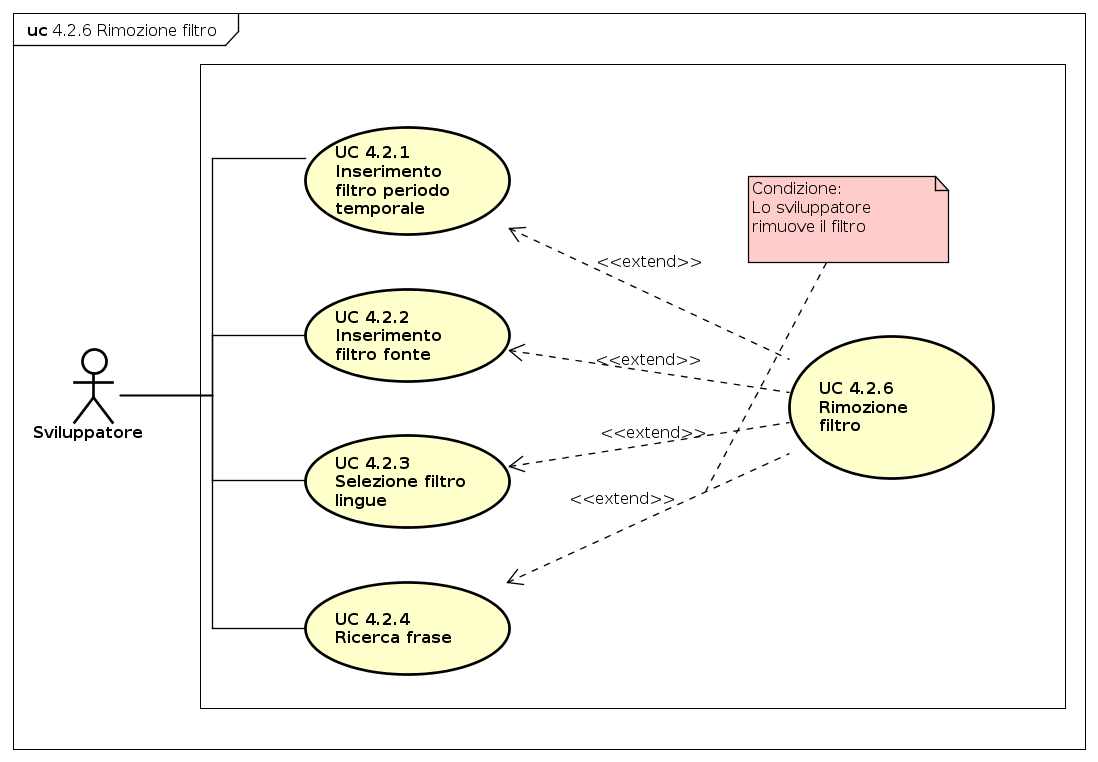
\includegraphics[width=17cm, height=10cm]{img/UC426.png} 
\caption{Caso d'uso UC 4.2.6 relativo alla rimozione dei filtri}\label{fig:426}
\end{figure}
\item[•]\textbf{Attori}: Sviluppatore;
\item[•]\textbf{Descrizione}: lo sviluppatore cancella il valore del filtro selezionato.
\item[•]\textbf{Precondizione}: il filtro contiene un valore ed è applicato un filtraggio ai dati rispettando le condizioni di tale filtro;
\item[•]\textbf{Postcondizione}: il filtro è stato rimosso pertanto i dati visualizzati non rispetteranno più tale vincolo;
\item[•]\textbf{Flusso degli eventi}: lo sviluppatore seleziona il filtro e lo rimuove.
 \end{itemize}

\subsubsection{UC 4.2.1.1 - Visualizzazione messaggio errore data errata}
\begin{itemize}
	\item[•]\textbf{Attori}: Sviluppatore;
	\item[•]\textbf{Descrizione}: lo sviluppatore visualizza un messaggio di errore sul periodo selezionato;
	\item[•]\textbf{Precondizione}: lo sviluppatore ha inserito una data non conforme all'interno del filtro relativo al periodo temporale;
	\item[•]\textbf{Postcondizione}: il filtro è stato erroneamente inserito pertanto viene visualizzato un messaggio di errore;
	\item[•]\textbf{Flusso degli eventi}: Lo sviluppatore inserisce una data non conforme e visualizza un errore.
\end{itemize}
\subsubsection{UC 4.2.4.1 - Visualizzazione messaggio errore input errato}
\begin{itemize}
	\item[•]\textbf{Attori}: Sviluppatore;
	\item[•]\textbf{Descrizione}: lo sviluppatore visualizza un messaggio di errore sulla ricerca.
	\item[•]\textbf{Precondizione}: lo sviluppatore ha inserito una frase non conforme;
	\item[•]\textbf{Postcondizione}: lo sviluppatore visualizza un messaggio di errore relativo all'inserimento di un input errato, cioè non conforme a ciò che il sistema si attendeva;
	\item[•]\textbf{Flusso degli eventi}: lo sviluppatore inserisce una frase non conforme e visualizza un errore.	
\end{itemize}

  
\subsubsection{UC 4.3 - Visualizzazione storico frase}
\begin{itemize}
\item[•]\textbf{Attori}: Sviluppatore;
\item[•]\textbf{Descrizione}: lo sviluppatore seleziona una frase dall'elenco e ne visualizza lo storico contenente la correzione fornita dal sistema automatico, ed eventualmente quelle redatte anche da insegnanti diversi;
\item[•]\textbf{Precondizione}: lo sviluppatore visualizza le frasi in base ai filtri stabiliti;
\item[•]\textbf{Postcondizione}: lo sviluppatore visualizza tutte le correzioni della frase;
\item[•]\textbf{Flusso degli eventi}: lo sviluppatore seleziona la frase e appare lo storico della frase.
\end{itemize}

\subsubsection{UC 4.4 - Scaricamento dati}
\begin{figure}[H]
\centering
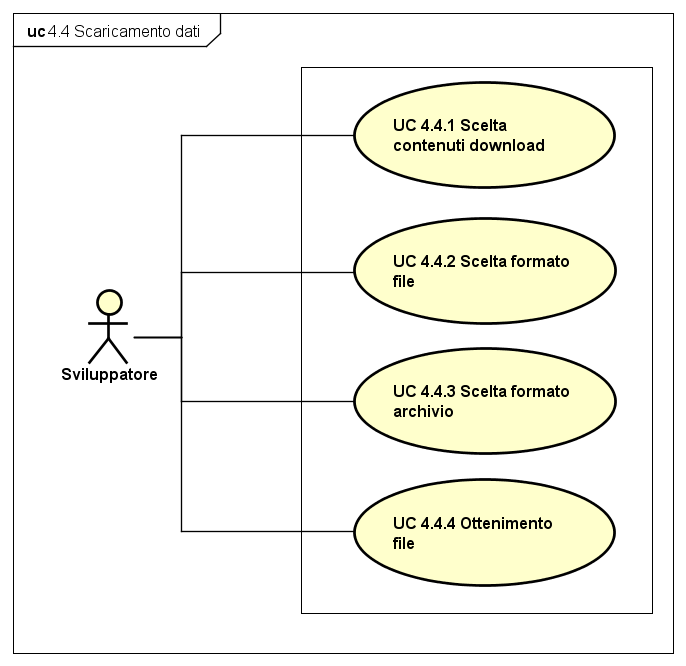
\includegraphics[width=17cm, height=10.5cm]{img/UC440.png} 
\caption{Caso d'uso UC 4.4}\label{fig:440}
\end{figure}
\begin{itemize}
\item[•]\textbf{Attori}: Sviluppatore;
\item[•]\textbf{Descrizione}: lo sviluppatore esegue il download dei dati d'interesse;
\item[•]\textbf{Precondizione}: lo sviluppatore visualizza i dati in ordine cronologico, e nel caso siano applicati filtri, vede solo i dati che rispettano tali filtri;
\item[•]\textbf{Postcondizione}: lo sviluppatore scarica un file contenente le analisi grammaticali in formato anonimo;
\item[•]\textbf{Flusso degli eventi}:
\begin{enumerate}
\item UC 4.4.1 - Scelta contenuti download;
\item UC 4.4.2 - Scelta formato file;
\item UC 4.4.3 - Scelta formato archivio;
\item UC 4.4.4 - Ottenimento file.
\end{enumerate}
\end{itemize}

\subsubsection{UC 4.4.1 - Scelta contenuti download}
\begin{itemize}
\item[•]\textbf{Attori}: Sviluppatore;
\item[•]\textbf{Descrizione}: lo sviluppatore sceglie gli elementi di interesse che vuole siano scaricati una volta completata la procedura di download;
\item[•]\textbf{Precondizione}: lo sviluppatore visualizza le preposizioni in base ai filtri stabiliti;
\item[•]\textbf{Postcondizione}: lo sviluppatore visualizza i contenuti che intende scaricare, come ad esempio lo storico di una frase;
\item[•]\textbf{Flusso degli eventi}: lo sviluppatore seleziona dall'elenco, eventualmente filtrato, le proposizioni d'interesse, come ad esempio quelle provenienti da i soli docenti selezionati.
\end{itemize}

\subsubsection{UC 4.4.2 - Scelta formato file}
\begin{itemize}
\item[•]\textbf{Attori}: Sviluppatore;
\item[•]\textbf{Descrizione}:  lo sviluppatore seleziona da un elenco prestabilito il formato dei file che intende scaricare;
\item[•]\textbf{Precondizione}: lo sviluppatore non ha stabilito il formato dei file che intende scaricare;
\item[•]\textbf{Postcondizione}: lo sviluppatore ha stabilito il formato dei file che intende scaricare;
\item[•]\textbf{Flusso degli eventi}: lo sviluppatore seleziona dall'elenco prestabilito un'opzione che determina il formato dei file che contengono i dati precedentemente scelti.
\end{itemize}

\subsubsection{UC 4.4.3 - Scelta formato archivio}
\begin{itemize}
\item[•]\textbf{Attori}: Sviluppatore;
\item[•]\textbf{Descrizione}: lo sviluppatore seleziona da un elenco prestabilito il formato dell'archivio compresso con cui vuole che i dati d'interesse siano compressi;
\item[•]\textbf{Precondizione}: il formato dell'archivio contenente i dati d'interesse non è definito;
\item[•]\textbf{Postcondizione}: il formato dell'archivio contenente i dati d'interesse è stato definito;
\item[•]\textbf{Flusso degli eventi}: lo sviluppatore seleziona dall'elenco prestabilito un'opzione che determina il formato dell'archivio che contiene i file relativi ai dati precedentemente scelti.
\end{itemize}


\subsubsection{UC 4.5 - Creazione modello}
\begin{figure}[H]
\centering
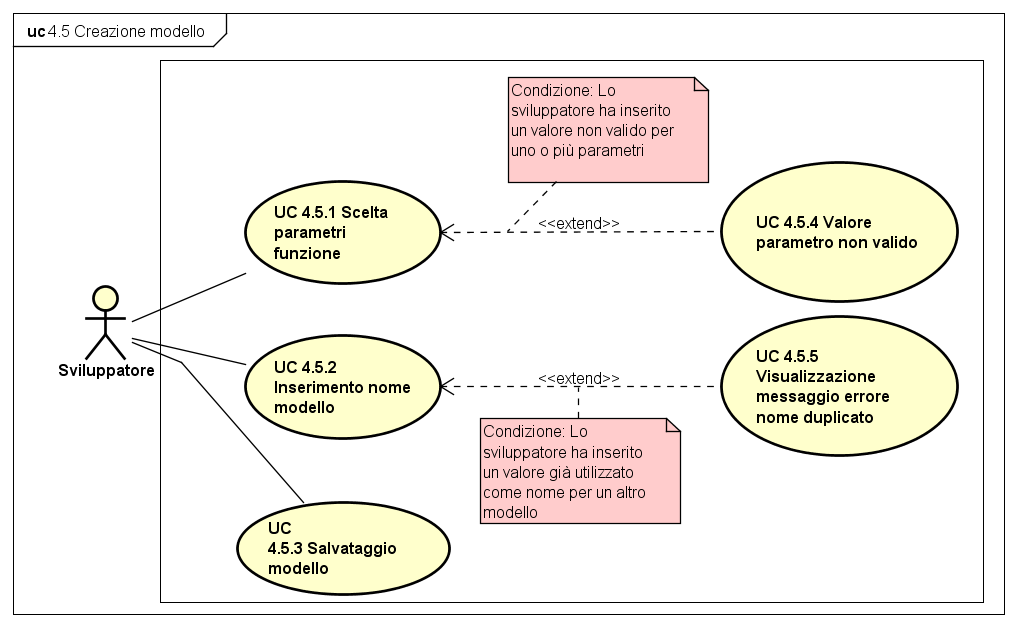
\includegraphics[width=17cm]{img/UC450.png} 
\caption{Caso d'uso UC 4.5}\label{fig:450}
\end{figure}
\begin{itemize}
\item[•]\textbf{Attori}: Sviluppatore;
\item[•]\textbf{Descrizione}: lo sviluppatore crea un nuovo modello;
\item[•]\textbf{Precondizione}: lo sviluppatore non ha creato il modello;
\item[•]\textbf{Postcondizione}: lo sviluppatore ha creato un nuovo modello;
\item[•]\textbf{Flusso degli eventi}:  
\begin{enumerate}
	\item UC 4.5.1 - Scelta parametri funzione;
	\item UC 4.5.2 - Inserimento nome modello;
	\item UC 4.5.3 - Salvataggio modello.
\end{enumerate}
\item[•]\textbf{Estensioni}:  
\begin{enumerate}
	\item UC 4.5.4 - Valore parametro non valido;
	\item UC 4.5.5 - Visualizzazione messaggio errore nome duplicato.
\end{enumerate}
\end{itemize}

\subsubsection{UC 4.5.1 - Scelta parametri funzione}
\begin{itemize}
\item[•]\textbf{Attori}: Sviluppatore;
\item[•]\textbf{Descrizione}: lo sviluppatore sceglie i parametri della funzione per la creazione di un nuovo modello con i relativi valori associati;
\item[•]\textbf{Precondizione}: lo sviluppatore non ha scelto i parametri da inserire;
\item[•]\textbf{Postcondizione}: lo sviluppatore ha inserito i parametri per la creazione di un nuovo modello;
\item[•]\textbf{Flusso degli eventi}:  lo sviluppatore inserisce tutti i parametri necessari che verranno impiegati nella realizzazione del modello.
\item[•] \textbf{Estensioni}: 
\begin{enumerate}
	\item UC 4.5.4 - Valore parametro non valido.
\end{enumerate}
\end{itemize}

\subsubsection{UC 4.5.2 - Inserimento nome modello}
\begin{itemize}
\item[•]\textbf{Attori}: Sviluppatore;
\item[•]\textbf{Descrizione}: lo sviluppatore inserisce il nome per il modello che intende salvare;
\item[•]\textbf{Precondizione}: lo sviluppatore non ha inserito il nome del modello;
\item[•]\textbf{Postcondizione}: lo sviluppatore ha inserito il nome del modello;
\item[•]\textbf{Flusso degli eventi}: lo sviluppatore inserisce una stringa che definisce il nome del modello che verrà memorizzato.
\item[•] \textbf{Estensioni}: 
\begin{enumerate}
	\item UC 4.5.5 - Visualizzazione messaggio errore nome duplicato.
\end{enumerate}
\end{itemize}

\subsubsection{UC 4.5.3 - Salvataggio modello}
\begin{itemize}
\item[•]\textbf{Attori}: Sviluppatore;
\item[•]\textbf{Descrizione}: lo sviluppatore salva il modello di cui ha definito il nome;
\item[•]\textbf{Precondizione}: lo sviluppatore ha inserito il nome del modello;
\item[•]\textbf{Postcondizione}: lo sviluppatore ha salvato il modello;
\item[•]\textbf{Flusso degli eventi}: lo sviluppatore seleziona l'opzione relativa al salvataggio che comporta il salvataggio del modello.
\end{itemize}

\subsubsection{UC 4.5.4 - Valore parametro non valido}
\begin{itemize}
\item[•]\textbf{Attori}: Sviluppatore;
\item[•]\textbf{Descrizione}: il sistema segnala un messaggio di errore relativo al valore del parametro non valido;
\item[•]\textbf{Precondizione}: lo sviluppatore ha inserito il valore del parametro;
\item[•]\textbf{Postcondizione}: lo sviluppatore visualizza un messaggio di errore relativo al valore del parametro non valido;
\item[•]\textbf{Flusso degli eventi}: lo sviluppatore inserisce un valore di parametro non valido e visualizza un errore.

\end{itemize}
\subsubsection{UC 4.5.5 - Visualizzazione messaggio errore nome duplicato}
\begin{itemize}
\item[•]\textbf{Attori}: Sviluppatore;
\item[•]\textbf{Descrizione}: lo sviluppatore visualizza un messaggio di errore relativo all'inserimento di un modello avente lo stesso nome di uno già inserito;
\item[•]\textbf{Precondizione}: lo sviluppatore ha inserito il nome del modello;
\item[•]\textbf{Postcondizione}: lo sviluppatore visualizza il messaggio di errore e inserisce un nuovo nome;
\item[•]\textbf{Flusso degli eventi}: lo sviluppatore inserisce un nome già presente nel sistema e visualizza un errore.
\end{itemize}

\subsubsection{UC 4.5.6 - Interruzione inserimento modello}
\begin{itemize}
\item[•]\textbf{Attori}: Sviluppatore;
\item[•]\textbf{Descrizione}: lo sviluppatore interrompe l'inserimento del modello, perdendo tutti i dati inseriti in precedenza;
\item[•]\textbf{Precondizione}: lo sviluppatore sta inserendo il modello;
\item[•]\textbf{Postcondizione}: nessun nuovo modello è stato inserito;
\item[•]\textbf{Flusso degli eventi}: lo sviluppatore interrompe l'inserimento del modello.
\end{itemize}

\subsubsection{UC 4.6 - Visualizzazione elenco modelli}
\begin{itemize}
\item[•]\textbf{Attori}: Sviluppatore;
\item[•]\textbf{Descrizione}: lo sviluppatore visualizza l'elenco dei propri modelli realizzati;
\item[•]\textbf{Precondizione}: lo sviluppatore si è autenticato nel sistema;
\item[•]\textbf{Postcondizione}: lo sviluppatore visualizza l'elenco dei propri modelli;
\item[•]\textbf{Flusso degli eventi}: lo sviluppatore seleziona la voce del menù relativa ai modelli e ne visualizza l'elenco.
\end{itemize}


\subsubsection{UC 4.7 - Visualizzazione contenuto modello} 
\begin{itemize}
\item[•]\textbf{Attori}: Sviluppatore;
\item[•]\textbf{Descrizione}: lo sviluppatore visualizza il contenuto del modello selezionato.
\item[•]\textbf{Precondizione}: lo sviluppatore visualizza l'elenco dei modelli;
\item[•]\textbf{Postcondizione}: lo sviluppatore visiona il contenuto del modello selezionato;
\item[•]\textbf{Flusso degli eventi}: lo sviluppatore seleziona un modello dall'elenco e ne visualizza il contenuto.
\end{itemize}

\subsubsection{UC 4.8 - Scaricamento modello}
\begin{itemize}
\item[•]\textbf{Attori}: Sviluppatore;
\item[•]\textbf{Descrizione}: lo sviluppatore ottiene un file contenente il modello precedentemente creato;
\item[•]\textbf{Precondizione}: lo sviluppatore visualizza il contenuto del modello che intende scaricare.
\item[•]\textbf{Postcondizione}: lo sviluppatore ottiene un file contenente il modello selezionato;
\item[•]\textbf{Flusso degli eventi}: lo sviluppatore seleziona l'opzione di scaricamento e ottiene un file contenente il modello.
\end{itemize}

\subsubsection{UC 4.9 - Eliminazione modello}
\begin{itemize}
	\item[•]\textbf{Attori}: Sviluppatore;
	\item[•]\textbf{Descrizione}: lo sviluppatore elimina il modello;
	\item[•]\textbf{Precondizione}: lo sviluppatore visualizza l'elenco dei propri modelli;
	\item[•]\textbf{Postcondizione}: lo sviluppatore ha eliminato il modello; 
	\item[•]\textbf{Flusso degli eventi}: 
	\begin{enumerate}
		\item Selezione modello;
		\item Selezione procedura eliminazione.
	\end{enumerate}   
\end{itemize}